\chapter{STRique Repeat Detection}
\label{sec:strique}

Expansions of short tandem repeats are genetic variants that have been implicated in several neuropsychiatric and other disorders, but their assessment remains challenging with current polymerase-based methods. Here we introduce a CRISPR-Cas-based enrichment strategy for nanopore sequencing combined with an algorithm for raw signal analysis. Our method, termed STRique for short tandem repeat identification, quantification and evaluation, integrates conventional sequence mapping of nanopore reads with raw signal alignment for the localization of repeat boundaries and a hidden Markov model-based repeat counting mechanism. We demonstrate the precise quantification of repeat numbers in conjunction with the determination of CpG methylation states in the repeat expansion and in adjacent regions at the single-molecule level without amplification. Our method enables the study of previously inaccessible genomic regions and their epigenetic marks.

\begin{figure}[h]
    \centering
    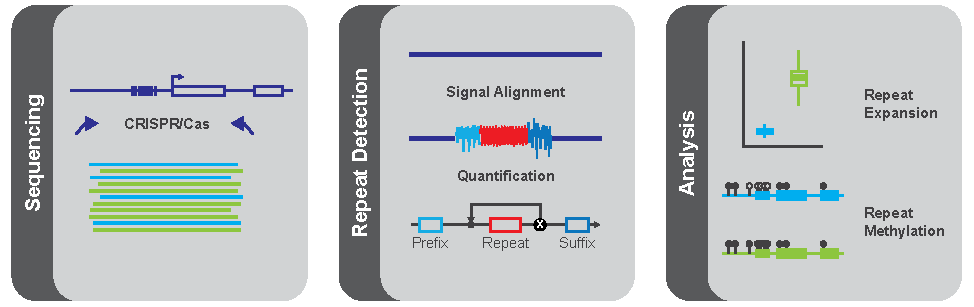
\includegraphics[width=1.0\textwidth]{figures/strique/GA.pdf}
    \label{fig:strique:ga}
\end{figure}




\section{Background}
\label{sec:strique:background}

The expansion of unstable genomic Short Tandem Repeats (STRs) causes more than 30 Mendelian human disorders.5 An extended GGGGCC-repeat $ [(G_{4}C_{2})_{n}] $ within the C9orf72 gene is the most frequent monogenic cause of Frontotemporal Dementia and Amyotrophic Lateral Sclerosis c9FTD/ALS.6 Similarly, accumulation of a CGG motif in the FMR1 gene underlies the Fragile X Syndrome, currently one of the most common identifiable genetic causes of mental retardation and autism.7 In both prototypical repeat expansion disorders, recent evidence has suggested pronounced inter- and intraindividual repeat variability as well as focal changes in DNA methylation to modulate the disease phenotype.8-10

To overcome current difficulties in characterizing expanded STRs we focused on three areas: i) optimization of nanopore sequencing and signal processing to capture STRs ii) development and implementation of a target enrichment strategy to increase efficiency and iii) integration of expansion measurements with CpG methylation at the single molecule level.
To enable a robust repeat analysis, we developed a general-purpose signal processing algorithm for the exact quantification of STR numbers in raw nanopore signals (STRique: Short Tandem Repeat identification, quantification \& evaluation, https://github.com/giesselmann/STRique). 


\section{Data Generation}
\label{sec:strique:data}



\section{Repeat Quantification}
\label{sec:strique:quantification}

To first benchmark existing repeat expansion counting methods we constructed, verified and nanopore sequenced plasmids with several synthetic $ [(G_{4}C_{2})_{n}] $-repeat lengths.16 Current (May 2019) production grade (Guppy v3.0.3) software developed by Oxford Nanopore Technologies (ONT) was used to translate the nanopore raw signal into base-space representations.

The analysis’ results revealed that the current generation of general-purpose basecalling algorithms cannot satisfactorily resolve expanded STR sequences (Supplementary Fig. 4). For our purpose we systematically combined outputs from three ONT basecaller generations (Albacore, Flappie, Guppy) and different parameter sets with two current sequence based STR quantification approaches (Decoy Alignment18 and RepeatHMM19, Fig. 1b). Albacore performed best with increased window size for the decoy alignment strategy while the high-accuracy model of Guppy provided the best sequence-derived results in combination with the RepeatHMM algorithm (Supplementary Fig. 4,5). Notably, we observed a systematic sequence strand bias resulting in more accurate counts for the GGGGCC sequence compared to the complementary strand (GGCCCC, Supplementary Fig. 5). We conclude, that the mentioned neural network basecallers, while enabling improved single read base quality on the genomic level,20 become unreliable for more than 32 (G4C2)n-repeats.
For overcoming these issues with our STRique signal analysis software (see Online Methods for details), first reads spanning a STR location are identified by aligning the conventionally base-called sequences to a reference.21 Next, STRique maps the upstream and downstream boundaries of each repeat more precisely with a signal alignment algorithm and, as a third step, quantifies the number of any given STR sequence with a Hidden Markov Model (HMM, Supplementary Fig. 3).22 Aggregated STRique repeat counts matched closely gel electrophoresis profiles (Bioanalyzer) from our synthetic repeat constructs and could be confirmed on the single molecule level by manually counting repeat patterns in raw signal traces (Fig. 1b,c, Supplementary Fig. 6,4).


Previously, repeat instability had been noted in Bacterial Artificial Chromosomes (BAC) containing expanded C9orf72 $ [(G_{4}C_{2})_{n}] $-repeats (Online Methods).17 Analysing BAC clone 239 from a c9FTD/ALS patient (G4C2)~800 (Ref. 17) with STRique, we observed STR contractions in many reads and a secondary peak at 800 repeats (Fig 1d, Online Methods), while all evaluated sequence space based methods failed to mirror previously published Southern blot results (Fig.1d, Supplementary Fig. 5). 17


Next, to establish a baseline reference data set, we performed nanopore sequencing of a whole genome library from c9FTD/ALS patient-derived DNA yielding a total of 29 Gbp from a single MinION flow cell. Consistent with approximately 10-fold genome-wide coverage, 10 reads covered the C9orf72 target region. To improve the coverage of any predetermined STR, but particularly the (G4C2)n-region in our proof of concept study, we took advantage of the programmable CRISPR-Cas12a-ribonucleoprotein (Cas12a-RNP), which cleaves DNA via staggered double-strand breaks.23 The Cas12a-RNP was first applied to selectively target DNA sequences from a patient-derived induced pluripotent stem cell line (24/5\#2) adjacent to the (G4C2)n-repeat resulting in unique 4 bp overhangs as molecular tags amenable to ligation of a linker oligo and subsequent attachment of the nanopore sequencing adapter (Fig. 2a: Workflow I, Online Methods). To further improve enrichment results we replaced the oligo adapter ligation step by adding Klenow fragment to fill in the Cas12a overhangs. The resulting dA-tailed DNA ends enabled even more efficient ligation of the sequencing adapters. In this enrichment protocol variant, the phosphorylated 5’-ends generated by Cas-nuclease mediated cleavage provide the molecular tag for selectively ligating the nanopore sequencing adaptors to the targeted DNA fragment (Fig. 2a, Workflow II).
Additional dephosphorylation of all 5’-ends before Cas12a-RNP-digestion chemically protects DNA ‘background’ fragments from being ligated to sequencing adapters. Consequently, only those fragments cut by Cas12a-RNPs are capable of being sequenced by this procedure (Fig. 2a). As a result, we were able to obtain up to 82 reads covering the (G4C2)n-repeat including 40 reads from the expanded allele from a single MinION flow cell (Supplementary Fig. 7, Supplementary Table 3, Supplementary Note). Strikingly, consistent with Southern blot results from the same cell line (Supplementary Fig. 8 a,b), we found two distinct repeat expansion distributions (Fig. 2b). To further explore the general applicability of our enrichment, sequencing and signal processing protocol to other repeat expansion disorders, we tested two isogenic, patient-derived cell lines (SC105iPS6, SC105iPS7) carrying distinct FMR1-repeat expansions.24 Employing an new set of FMR1-targeting Cas12a-RNPs (Supplementary Table 1) we found two different repeat expansion distributions as predicted by Southern blot analysis (Fig. 2c, Supplementary Fig. 8 c,d).
Since other CRISPR/Cas-nucleases also generate phosphorylated 5’-ends after DNA cleavage,25 we explored, if nucleases such as Cas9 might enable additional improvements of the enrichment results. Therefore, we prepared libraries in parallel with Cas12a- and Cas9-RNPs targeting both FMR1 and C9orf72 regions. Remarkably Cas9-targeting results in an additional increase in sequencing depth in the order of a magnitude for both targeted regions concomitant with a notable reduction in off-target reads (Fig. 2d, Supplementary Fig. 7c). To understand, if the number of reads on target can be further improved by exposing the same Cas12a- or Cas9- enrichment library to an increased number of pores, we subjected equimolar aliquots from the same pooled library preparations from Fig. 2b to nanopore sequencing on PromethION flow cells, which contain on average six times as many nanopores. However, we did not observe a gain in reads on target with the larger flow cells (Supplementary Fig. 7c).



\begin{figure}[h]
    \centering
    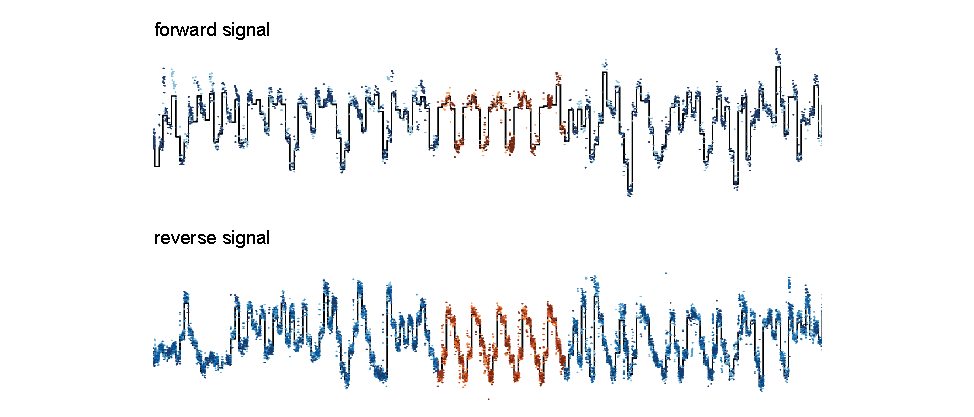
\includegraphics[width=1.0\textwidth]{figures/strique/signal.pdf}
    \captionsetup{format=plain}
    \caption[Nanopore raw signal of the C9orf72 STR in NA12878 cells]{Compound multi signal HMM alignment of publicly available raw traces from two template and eight complement reads from the NA12878 cell line shows matching signal pattern in all reads \cite{Jain2018}. Displayed are the current measurements as dots and the model signal as black line. Blue dots indicate current measurements identified as prefix or suffix sequence. Red dots indicate raw current measurements identified by STRique as belonging to the C9orf72-$ (G_{4}C_{2})_{n} $-STR. STRique detects in this case a $ (G_{4}C_{2})_{5} $-repeat.}
    \label{fig:strique:signal}
\end{figure}

\begin{figure}[h]
    \centering
    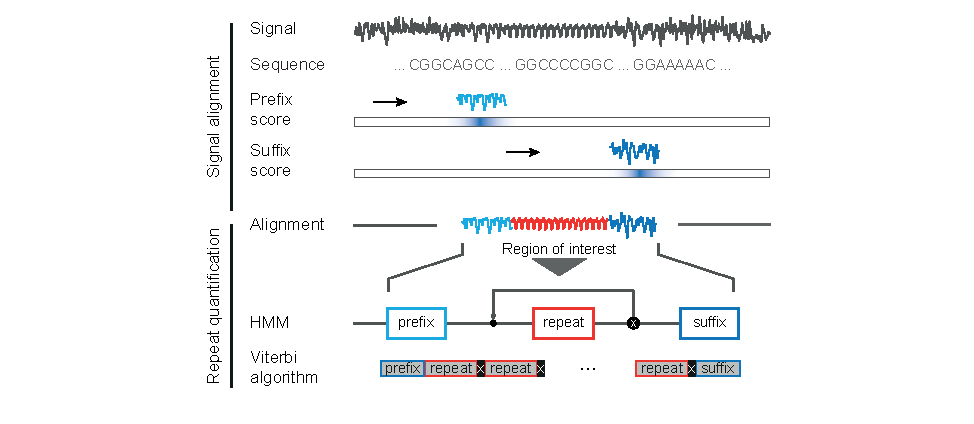
\includegraphics[width=1.0\textwidth]{figures/strique/count_structure_plasmid.pdf}
    \captionsetup{format=plain}
    \caption[STRique: generic repeat detection pipeline on raw nanopore signals.]{\textbf{a}, Repeat quantification enabled by raw signal alignment of flanking prefix and suffix regions and HMM-based count on the signal of interest. \textbf{b}, Bioanalyzer electropherogram, decoy alignment, RepeatHMM and STRique counts of synthetic $ (G_{4}C_{2})_{n} $ repeats.}
    \label{fig:strique:count_structure_plasmid}
\end{figure}

\begin{figure}[h]
    \centering
    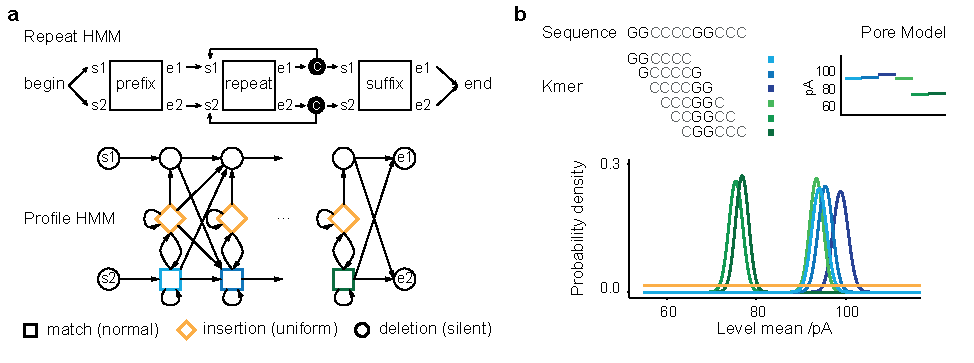
\includegraphics[width=1.0\textwidth]{figures/strique/count_hmm.pdf}
    \captionsetup{format=plain}
    \caption[Nanopore signal processing with STRique]{\textbf{a}, A compound profile HMM of prefix, a single repeat and the suffix sequence assigns either prefix, repeat or suffix label to each signal value. Repeat counts are obtained through dummy states between repeat and suffix. \textbf{b}, Nanopore signal profile HMM with normal distributed match state and uniform distributed insertion state emission probabilities.}
    \label{fig:strique:count_hmm}
\end{figure}

\begin{figure}[h]
    \centering
    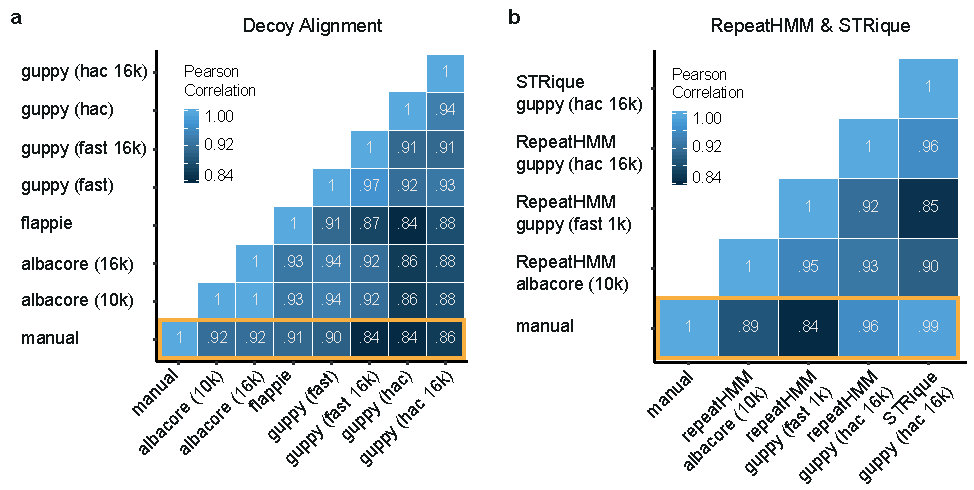
\includegraphics[width=1.0\textwidth]{figures/strique/count_sequence_corr.pdf}
    \captionsetup{format=plain}
    \caption[Correlation of sequence based STR detection methods]{\textbf{a}, Correlation of manual counted repeat lengths with sequence base methods. Decoy alignment against reference with 3-100 repeats with Albacore (window 10k and 16k), Guppy (fast and hac mode, 1k and 16k window size) and Flappie base-calling (n=204 reads). \textbf{b}, Correlation of manual count with RepeatHMM and STRique results (n=204 reads).}
    \label{fig:strique:count_sequence_corr}
\end{figure}

\begin{figure}[h]
    \centering
    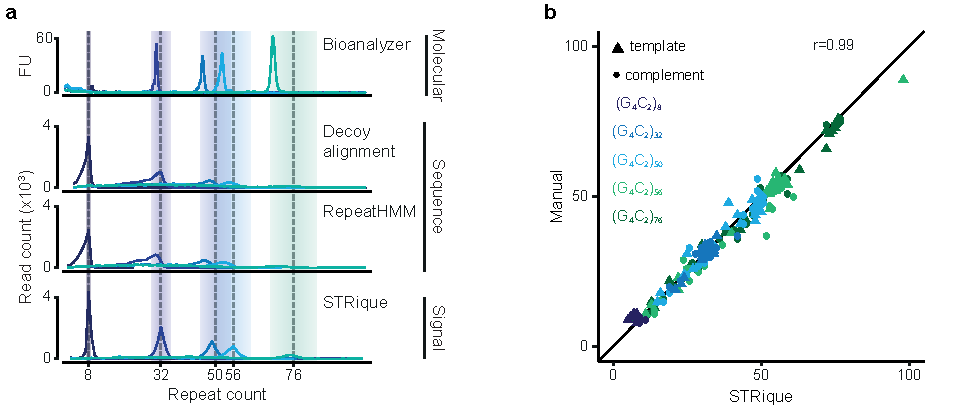
\includegraphics[width=1.0\textwidth]{figures/strique/count_signal_corr.pdf}
    \captionsetup{format=plain}
    \caption[Correlation and strand bias in STR analysis methods]{Manual counted set of plasmid reads on y-axis correlating with guppy base-calling and decoy alignment approach, RepeatHMM and STRique raw signal pipeline on x-axis. Only data points shown which could be evaluated with all four methods (n=15, 49, 45, 48, 47; Pearson correlation).}
    \label{fig:strique:count_signal_corr}
\end{figure}

\begin{figure}[h]
    \centering
    \includegraphics[width=1.0\textwidth]{figures/strique/count_bac.pdf}
    \captionsetup{format=plain}
    \caption[Strand bias in sequence based repeat counts]{Comparison of repeat counts from STRique, decoy alignment based on guppy (high accuracy model, 16k window size) and repeatHMM based on guppy (high accuracy model, 16k window size) for BAC data. One dot (n=5004) per read passing all three approaches and colored by strand.}
    \label{fig:strique:count_bac}
\end{figure}

\begin{figure}[h]
    \centering
    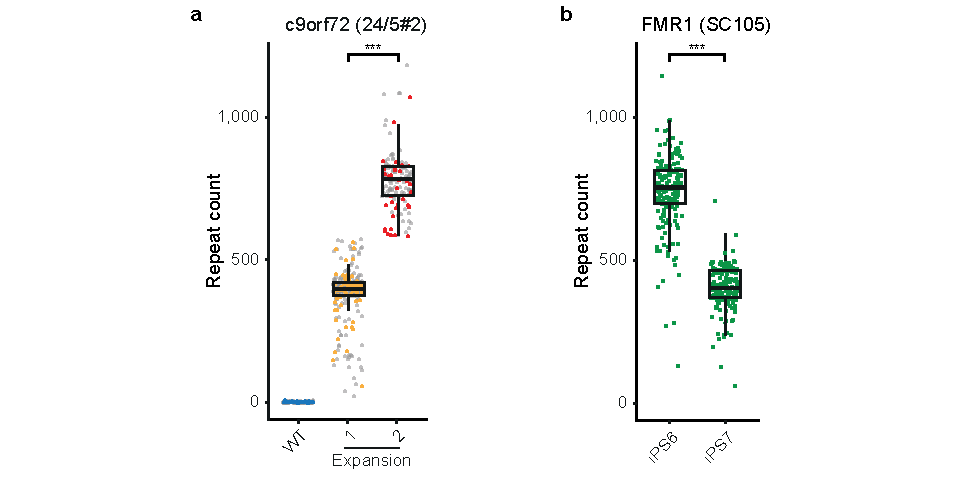
\includegraphics[width=1.0\textwidth]{figures/strique/count_patient_samples.pdf}
    \captionsetup{format=plain}
    \caption[Repeat quantification in c9orf72 and FMR1 patients]{\textbf{a}, Repeat quantification of sample 24/5\#2 at the C9orf72 locus, revealing two distinct repeat bands of ~450 and ~750 $ (G_{4}C_{2})_{n} $ repeats (n = 1,810, 738 and 363 evaluated reads with a difference in repeat length of 392 (95\% confidence interval (CI): 383 to 400), $ P < 2.2 \cdot 10^{-16} $). Colored points indicate reads used in Fig. \ref{fig:strique:methylation_c9orf72_region}b. WT, wild type. \textbf{b}, Repeat quantification of the SC105iPS6 and SC105iPS7 samples at the FMR1 locus (n = 174 and 168 evaluated reads with a difference in repeat length of -343 (95\% CI: -361 to -325), $ P < 2.2 \cdot 10^{-16} $). P values in a and b were obtained by a two-sided Wilcoxon rank-sum test; $ ***P < 0.001 $. Data are presented as boxplots (centerline, median; box limits, first and third quartiles; whiskers, 1.5x interquartile range).}
    \label{fig:strique:count_patients}
\end{figure}

\begin{figure}[h]
    \centering
    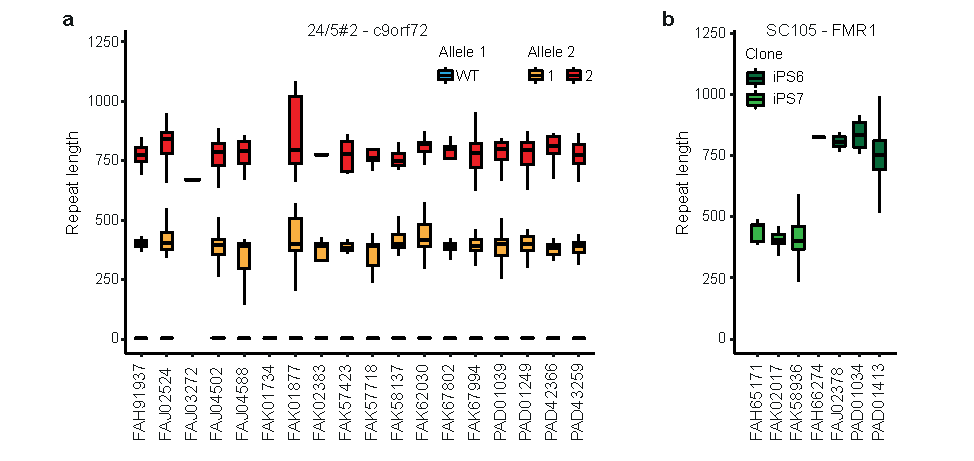
\includegraphics[width=1.0\textwidth]{figures/strique/count_experiments.pdf}
    \captionsetup{format=plain}
    \caption[Repeat count cluster stability over experiments]{\textbf{a}, C9orf72 target enrichment flow cells for patient 24/5\#2 \textbf{b}, FMR1 enrichment flow cells of SC105iPS6/iPS7. (FA*: MinION, PAD*: PromethION, number of reads per boxplot are in Supplementary Tables 5-6 column wt and exp). Data presented as boxplots (centerline, median; box limits, first and third quartiles; whiskers, 1.5x interquartile range; outliers not shown)}
    \label{fig:strique:count_experiments}
\end{figure}




\section{Base Modification Detection}
\label{sec:strique:modifications}

The epigenetic modification of C9orf72 and FMR1 loci have been correlated with STR expansion status and patient characteristics in both disorders, however without quantification at the single molecule level so far.10,26 Therefore we integrated single read CpG methylation analysis of regions adjacent to both STRs using nanopolish14 with our STRique results (Fig. 3a). We found that in the 24/5\#2 line all reads with STR expansions > 750 repeats showed a significantly increased methylation level at the promoter CpG island. In contrast all wild type reads and those with ~450 repeats were not or only partially methylated (Two sided Wilcoxon rank sum test p < 0.001, Fig. 3b, Supplementary Fig. 9, Supplementary Note).
Additionally, in c9FTD/ALS patients pervasive CpG methylation of the (G4C2)n-repeat itself has been reported.27 Assessed with a strictly qualitative assay, the expanded STR itself was reported to be methylated in the majority of cases examined.27 A similar observation has been directly implicated in the pathogenesis of FXS, where a CGG repeat expansion at the FMR1-locus beyond a threshold of > 200 repeats leads in most cases to the silencing of the entire FMR1-gene through CpG-methylation.28
Due to the intrinsic heterogeneity in STR length, especially reference genome based methods such as nanopolish14 cannot be used to determine CpG methylation on the repeat expansion itself. To detect 5mC modifications on STRs, we extended STRique by employing a parallel HMM with unmodified- and 5mC-paths. This single read analysis returns a methylation state for each tandem repeat, which then can be summarized into the mean repeat methylation level over the whole repetitive sequence.
When applying the methylation-aware STRique, all expanded FMR1-STRs in nanopore reads from patient SC105 are found to be highly methylated (Supplementary Fig. 10a), consistent with previous analyses29 and our Southern blot results (Supplementary Fig. 8). We next evaluated this approach on plasmids containing n=76 synthetic (G4C2)n and n=99 CGG-repeats (Addgene, \#63089), which were covalently modified with the methyltransferase M.SssI (Supplementary Fig. 10).14 In addition we tested the algorithm on (G4C2)n-containing reads (online methods) from patient-derived DNA, which had been modified with M.SssI in vitro. In summary, we found that STRique can determine the repeat CpG methylation state correctly in all positive and negative controls evaluated.
Surprisingly though, all reads covering the C9orf72-STR from our patient-derived samples showed little to no CpG-methylation, independently of the repeat expansion length or methylation status of the promoter CGI (Fig. 3b).


\begin{figure}[h]
    \centering
    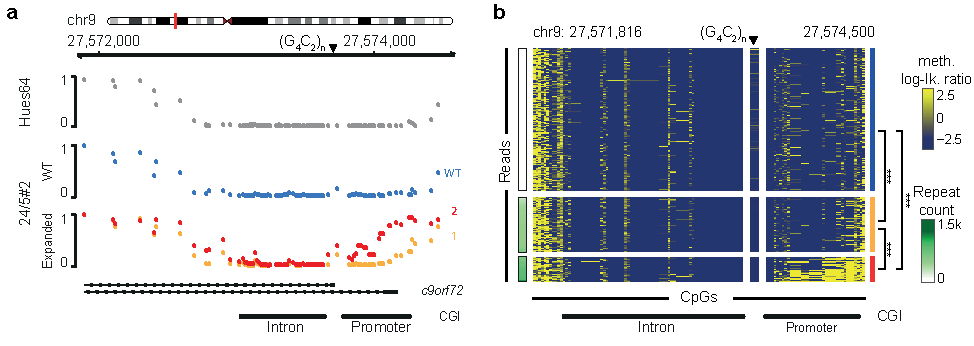
\includegraphics[width=1.0\textwidth]{figures/strique/methylation_c9orf72_region.pdf}
    \captionsetup{format=plain}
    \caption[Methylation state analyses at the single-read level]{\textbf{a}, C9orf72 methylation status in HUES64 as measured by whole-genome bisulfite sequencing. The wild-type (blue) allele and expanded (ex; orange) alleles (with 450 and 750 $ (G_{4}C_{2})_{n} $ repeats (red), respectively) are shown for patient 24/5\#2, as measured by nanopore sequencing. \textbf{b}, Single read nanopore methylation of C9orf72 covering reads from the minus strand (n = 259, 100 and 43 rows per block) sorted by detected repeat length (rows, single read; columns, single CpGs). CpGs with logP ratio $> 2.5$ are considered methylated, while those with logP ratio $< -2.5$ are considered unmethylated. The median methylation difference (95\% CI) and P value (determined by two-sided Wilcoxon rank-sum test on mean promoter CGI methylation) for comparisons were as follows: $ WT-ex450: 3.9 \cdot 10^{-5} (4.8 \cdot 10^{-6} to 3.4 \cdot 10^{-2}), P = 5.3 \cdot 10^{-9}; WT-ex750: 0.56 (0.46-0.64), P < 2.2 \cdot 10^{-16}; ex450-ex750: 0.53 (0.40-0.64), P < 2.2 \cdot 10^{-16}; ***P < 0.001. $ }
    \label{fig:strique:methylation_c9orf72_region}
\end{figure}

\begin{figure}[h]
    \centering
    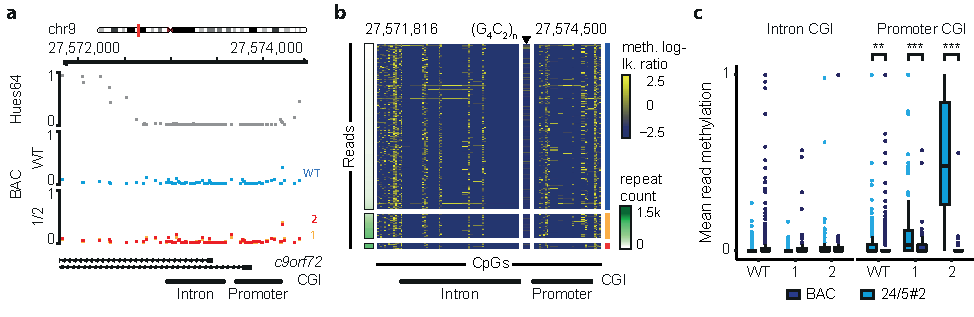
\includegraphics[width=1.0\textwidth]{figures/strique/methylation_bac_region.pdf}
    \captionsetup{format=plain}
    \caption[Nanopore single read methylation in BAC data]{\textbf{a}, Methylation status of c9orf72 region in BAC data for repeats < 200 (WT), 200-750 (Cluster1,orange) and > 750 (Cluster2,red) and control (Hues64, WGBS) \textbf{b}, Single read methylation on a sample of 500 BAC minus strand reads sorted by repeat count (row split 200 and 750 repeats, n=423,63,14). \textbf{c}, Difference in mean CGI methylation of intron and promoter per read on minus strand. Reads binned by detected repeat length for BAC (n=2066 WT; 315 Cluster1; 72 Cluster2) and patient 24/5\#2 (n=925 WT; 362 Cluster1; 153 Cluster2). Two sided Wilcoxon rank sum test, corrected for multiple testing (Holm), q-vals: * 0.05 - 0.01; ** 0.01 - 0.001; *** < 0.001. Median methylation differences between promoter CGI [95\%CI] for WT $-2.3e^{-5} [CI: -5.6e^{-6}:-1.5e^{-5}, q=7.4e^{-3}] $ and Cluster1 $ -0.01 [CI: -7.1e^{-5}:-3.4e^{-2}, q=1.4e^{-17}] $ and Cluster2 $ -0.46 [CI: -0.58:-0.37, q=1.0e^{-26}] $.}
    \label{fig:strique:methylation_bac_region}
\end{figure}

\begin{figure}[h]
    \centering
    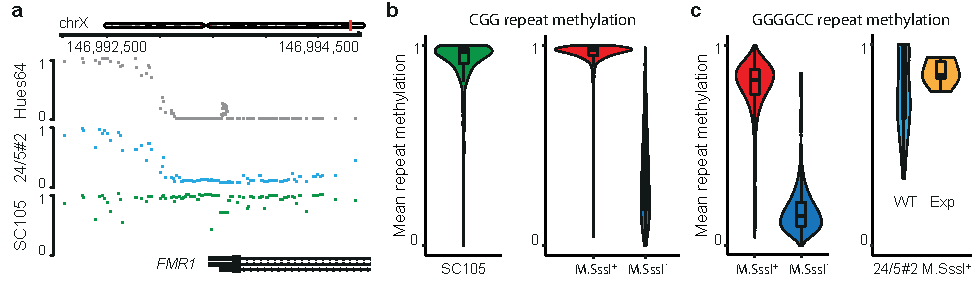
\includegraphics[width=1.0\textwidth]{figures/strique/methylation_repeat.pdf}
    \captionsetup{format=plain}
    \caption[Region and repeat methylation detection]{\textbf{a}, FMR1 region methylation in SC105iPS6/iPS7 compared to Hues64 WGBS and patient sample 24/5\#2. \textbf{b}, CGG mean repeat methylation status detected by STRique for SC105 (n=197) and synthetic plasmid control with 99 repeats treated with $ M.SssI^{+/-} $ (5mC level on minus strand, n=1232 $ M.SssI^{+} $; n=11991 $ M.SssI^{-} $). \textbf{c}, GGGGCC repeat methylation status for plasmid control with 76 repeats treated with $ M.SssI^{+/-} $ (n=2939 $ M.SssI^{+} $; n=31280 $ M.SssI^{-} $) and patient sample 24/5\#2 treated with $ M.SssI^{+} $ (5mC level on minus strand, n=52 WT and n=6 Cluster1). Data in (b-c) presented as violin plots with overlayed boxplots (centerline, median; box limits, first and third quartiles; whiskers, 1.5x interquartile range; outliers not shown).}
    \label{fig:strique:methylation_repeat}
\end{figure}




\section{Summary}
\label{sec:strique:summary}

Our results demonstrate the precise and multi-layered molecular characterization of pathological short tandem repeat expansions. We have increased the enrichment for regions of interest on the background of the human genome approximately two orders of magnitude without any target amplification by using selective, multiplexed CRISPR/Cas-nuclease-based chemical tagging of DNA fragments. Importantly, our method does not require any additional instruments in contrast to other previously reported30 enrichment strategies and enables reporting the DNA methylation status of the same alleles. The CRISPR/Cas-nuclease-target enrichment and STRique can be rapidly adapted to any other genomic region of interest, ensuring broad applicability to overcome challenges associated with the single molecule analysis. This allows for immediate integration of genetic and epigenetic signals associated with unstable repeat expansions or any other as of yet unsequenceable genomic regions in human health and disease. This type of analysis improves diagnostic workflows in regard to accuracy and resolution of unstable repeat expansion while enabling efforts to gain mechanistic insights into effects on differentiation, aging and future therapeutic agents that modify DNA methylation.


